\documentclass[../kl10.tex]{subfiles}
\graphicspath{{\subfix{../images/}}}



\begin{document}

\section{Kohlensäure - wenn Gase sauer werden}

Kolbi bleibt sehr gut hydriert und trinkt dafür für sein Leben gern Sprudelwasser. Dieses bekommt er meistens aus seiner eigenen Wassersprudelmaschine, die er sich mit seinem Freund Physli zusammengebastelt hat. Jetzt interessiert er sich natürlich dafür, wie sauer das Wasser ist, das er mit \ce{CO2} versetzt und so gerne trinkt. Als Erstes überlegt er sich, wie die Kohlensäure in sein Wasser kommt.

\enumaufgabe{\operator{Gib} die Reaktionsgleichungen für die Reaktion von \ce{CO2} mit Wasser und die darauffolgenden möglichen Dissoziationsstufen \operator{an}.}
\solution{
I) \ce{CO2 + H2O <=> H2CO3}\\
II) \ce{H2CO3 + H2O <=> HCO3- + H3O+} bzw. \ce{H2CO3 <=> HCO3- + H+}\\
\ce{HCO3- + H2O <=> CO3^2- + H3O+} bzw. \ce{HCO3- <=> CO3^2- + H+}\\
jeweils 1 P. \\Insg. 3P.
}{3cm}

\enumaufgabe{\operator{Gib} die Strukturformel für Natriumhydrogencarbonat \operator{an}.}
\solution{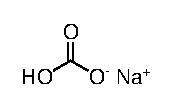
\includegraphics[width=0.3\textwidth]{2024/Abbildungen/Kohlensäure/NaHCO3.eps}
1 P.}{3cm}


Zum Untersuchen des Mineralwassers, welches er aufsprudelt, kauft Kolbi sich im Supermarkt zwei verschiedene Flaschen stilles Wasser.
Bevor er sich den Experimenten widmet, schaut sich Kolbi die beiden Wasserflaschen an und entdeckt folgende Mineralstoffangaben:

\begin{table}[H]
    \centering
    \begin{tabular}{l|c|c}
         Ion & Flasche 1 & Flasche 2  \\\hline
         Natrium & 13,5\thinspace mg/L  & 23,4\thinspace mg/L  \\\hline
         Kalium & 1,3\thinspace mg/L  &  5,7\thinspace mg/L \\\hline
         Calcium & 70,4\thinspace mg/L  &  439,0\thinspace mg/L \\\hline
         Fluorid & 0,15\thinspace mg/L  & /  \\\hline
         Chlorid & 21\thinspace mg/L  &  9,8\thinspace mg/L \\\hline
         Nitrat & <0,3\thinspace mg/L  & /  \\\hline
         Sulfat & 27\thinspace mg/L  &  1140,0\thinspace mg/L \\\hline
         Hydrogencarbonat & 342\thinspace mg/L  & 292,0\thinspace mg/L  \\
    \end{tabular}
\end{table}

Beim Versetzen der beiden Mineralwasser mit einem Überschuss von Natronlauge tritt jeweils ein weißer Niederschlag auf.

\newpage

\enumaufgabe{\operator{Begründe} basierend auf den Mineralstoffangaben und anhand von Reaktionsgleichungen, um welchen Stoff es sich handelt.}
\solution{In den beiden Lösungen liegen \ce{Ca^2+} und \ce{HCO3-} vor.\\
Nach Zugabe Natronlauge wird \ce{HCO3-} deprotoniert: \ce{HCO3- + NaOH -> CO3^2- + H2O + Na+} \\
Diese fält zusammen mit \ce{Ca^2+} als Calciumcarbonat aus: \ce{Ca^2+ +CO3^2 -> CaCO3 v} \\
Alle anderen Ionenkombinationen würden nicht ausfallen\\
jeweils 1 P. für die beiden Gleichungen und \ce{CaCO3} als NS\\
insg. 3 P.}{4cm}



\enumaufgabe{\operator{Berechne} die Masse $m$ des Niederschlags, die jeweils aus  $1,5\ \si{L}$ großen Flaschen des Wassers ausfallen kann unter der Annahme, dass das Produkt vollständig ausfällt.\\
Hinweis: Solltest du bei Teilaufgabe c) kein Ergebnis haben, gehe davon aus, dass \ce{Na2SO4} gefällt wird.}
\solution{
Flasche 1:
$$n_{\rm Ca^{2+}}=\frac{\beta_{\rm Ca^{2+}}\cdot V}{M_{\rm Ca^{2+}}}=\rm\frac{70,4\frac{mg}{L}\cdot1,5\thinspace L}{40,078\frac{g}{mol}}=2,635\thinspace mmol\qquad 1 P.$$
$$n_{\rm CO_3^{2-}}=\frac{\beta_{\rm HCO_3^{-}}\cdot V}{M_{\rm HCO_3^{-}}}=\rm\frac{342\frac{mg}{L}\cdot1,5\thinspace L}{61,017\frac{g}{mol}}=8,407\thinspace mmol\qquad 1 P.$$
$$\Rightarrow n_{\rm CaCO_3}=n_{\rm Ca^{2+}}\qquad 0,5 P.$$
$$m_{\rm CaCO_3}=n_{\rm CaCO_3}\cdot M_{\rm CaCO_3}=\rm2,635\thinspace mmol\cdot100,09\frac{g}{mol}=\underline{\underline{263,7\thinspace mg}}\qquad 1 P.$$
Flasche 2:
$$n_{\rm Ca^{2+}}=\frac{\beta_{\rm Ca^{2+}}\cdot V_{\rm Ca^{2+}}}{M_{\rm Ca^{2+}}}=\rm\frac{439,0\frac{mg}{L}\cdot1,5\thinspace L}{40,078\frac{g}{mol}}=16,43\thinspace mmol\qquad 1 P.$$
$$n_{\rm CO_3^{2-}}=\frac{\beta_{\rm HCO_3^{-}}\cdot V}{M_{\rm HCO_3^{-}}}=\rm\frac{292,0\frac{mg}{L}\cdot1,5\thinspace L}{61,017\frac{g}{mol}}=7,178\thinspace mmol\qquad 1 P.$$
$$\Rightarrow n_{\rm CaCO_3}=n_{\rm CO_3^{2-}}\qquad 0,5 P.$$
$$m_{\rm CaCO_3}=n_{\rm CaCO_3}\cdot M_{\rm CaCO_3}=\rm7,178\thinspace mmol\cdot100,09\frac{g}{mol}=\underline{\underline{718,4\thinspace mg}}\qquad 1 P.$$
Alternativergebnis: Flasche 1: 59,89\thinspace mg; Flasche 2: 108,4\thinspace mg (hier Faktor 2 von \ce{Na+} beachten)\\
Folgefehler geben; insg. 7 P.
}{9.5cm}


Um den \ce{CO2}-Gehalt von seinen zu Hause gesprudelten Wasserflaschen zu bestimmen, titriert Kolbi dieses Wasser mit Natronlauge. Für die Maßlösung wurden 1,000\thinspace g Natriumhydroxid in 500,0\thinspace mL Wasser gelöst. Der Verbrauch an Natronlauge bis zum ersten Umschlagspunkt betrug im Schnitt 9,543\thinspace mL bei 10,00\thinspace mL Wasserprobe.

\newpage

\enumaufgabe{\operator{Berechne} die Stoffmenge an Kohlenstoffdioxid, die man aus einer $\SI{1,5}{\liter}$-Flasche der Analysenlösung austreiben könnte. \operator{Gib} auch das Volumen an \ce{CO2} \operator{an}, das bei $\SI{101,325}{\kilo\pascal}$ und \SI{25}{\celsius} dabei frei würde.}
\solution{
\ce{H2CO3 + NaOH -> HCO3- + H2O + Na+} oder \ce{CO2 + NaOH -> HCO3- + Na+} \\ 0,5 P. für 1:1 Stöchiometrie, Reaktionsgleichung nicht zwingend erforderlich\\
$$c_{\rm NaOH}=\frac{m_{\rm NaOH}}{M_{\rm NaOH}\cdot V_{Lsg}}=\rm\frac{1,00\thinspace g}{39,99707\frac{g}{mol}\cdot 0,500\thinspace L}=0,05000\frac{mol}{L}\qquad 1 P.$$
$$c_{\rm H_2CO_3}\cdot V_{\mathrm{L}}=c_{\rm NaOH}\cdot V_{\mathrm{M}}\qquad \mathrm{0,5 P.}$$
$$c_{\rm H_2CO_3}=\rm\frac{0,05000\frac{mol}{L}\cdot9,54\thinspace mL}{10,0\thinspace mL}=0,0477\frac{mol}{L}\qquad 1 P.$$
$$n_{\rm CO_2}=n_{\rm H_2CO_3}=c_{\rm H_2CO_3}\cdot V_{\mathrm{Flasche}}=\rm0,0477\frac{mol}{L}\cdot1,5\thinspace L=\underline{\underline{0,0716\thinspace mol}}\qquad 1 P.$$
$$pV=nRT\qquad 0,5 P.$$
$$V_{\rm CO_2}=\frac{n_{\rm CO_2}\cdot R\cdot T}{p}=\rm\frac{0,0716\thinspace mol\cdot 8,314\frac{J}{K\cdot mol}\cdot 298,15\thinspace K}{101,325\thinspace kPa}=\underline{\underline{1,75\thinspace L}}\qquad 1 P.$$
insg. 5,5 P.}{7cm}





In der Schule überlegt sich Kolbi, was für einen Effekt seine ganzen Wasserflaschen auf die \ce{CO2}-Konzentration des Klassenzimmers haben könnten. 
Sein Klassenzimmer besitzt eine Länge von 8,0\thinspace m, eine Breite von 6,0\thinspace m und ist 2,7\thinspace m hoch. Die Luft besteht zu 420,0 ppm (Teile pro Million) aus \ce{CO2}.


\enumaufgabe{\operator{Berechne}, aus wie vielen Wasserflaschen aus Teilaufgabe e) man das \ce{CO2} austreiben und in den Raum einleiten müsste, um den \ce{CO2}-Gehalt bei $\SI{101,325}{\kilo\pascal}$ und \SI{25}{\celsius} zu verdoppeln. Berücksichtige dabei die Gesamtstoffmengenänderung der Luftmoleküle im Klassenzimmer und nimm an, dass das Klassenzimmer ein isochores System ist.\\
Hinweis: Solltest du Teilaufgabe e) nicht gelöst haben, rechne mit einer Stoffmenge von $\SI{0,1}{\mole}\ \ce{CO2}$ in jeder Flasche.}
\solution{
$$V_{\rm Zimmer}=a\cdot b\cdot h=\rm129,6\thinspace m^3\qquad 1 P.$$
$$pV=nRT$$
$$n_{\rm Luft}=\frac{p\cdot V_{\rm Zimmer}}{R\cdot T}=\rm\frac{101325\thinspace Pa\cdot 129,6\thinspace m^3}{8,314\frac{J}{K\cdot mol}\cdot298,15\thinspace K}=5298\thinspace mol\qquad 1 P.$$
$${\rm (I)\ }n_{\rm Luft}+n_{\rm CO_2, e}=n_{\rm ges}$$
$${\rm (II)\ }n_{ges}\cdot 0,084\%=n_{\rm CO_2, g}$$
$${\rm (III)\ }n_{\rm CO_2, g}-n_{\rm Luft}\cdot 0,042\%=n_{\rm CO_2, e}$$
$$\Rightarrow n_{\rm CO_2, e}=\frac{0,00042\cdot n_{\rm Luft}}{1-0,00084}=\frac{0,00042\cdot 5298\thinspace\rm mol}{0,99916}=\rm2,227\thinspace mol$$\text{3 P. (davon 1,5 P. für Gleichungssystem)}
$$\frac{n_{\rm CO_2, e}}{n_{\mathrm{CO_2, Flasche}}}=\rm\frac{2,227\thinspace mol}{0,0716\thinspace mol}=\underline{\underline{31,10\ Flaschen}}\qquad 1 P.$$
Alternativwert: 22,27 Flaschen\\
insg. 6 P.
}{8.3cm}

\newpage

\enumaufgabe{\operator{Berechne} die daraus resultierende Druckzunahme unter der Annahme, dass das Klassenzimmer ein isochores System ist.\\Hinweis: Solltest du Teilaufgabe f) nicht gelöst haben, rechne mit $30$ Flaschen à $\SI{0,1}{\mole}\ \ce{CO2}$.}
\solution{
$$pV=nRT$$
$$p_{\rm CO_2}=\frac{n_{\rm CO_2}\cdot R\cdot T}{V_{\rm Raum}}=\rm\frac{2,227\thinspace mol\cdot8,314\frac{J}{K\cdot mol}\cdot298,15\thinspace K}{129,6\thinspace m^3}=\underline{\underline{42,60\thinspace Pa}}$$
Alternativergebnis: 57,38\thinspace Pa\\
insg. 1,5 P.}{3cm}
\solutiontext{$\sum$ 27 P.}{}



\end{document}